\documentclass{article}
\usepackage[utf8]{inputenc}
\usepackage[czech]{babel}
\usepackage[dvipsnames]{xcolor}

\usepackage{graphicx}
\usepackage{ulem,amsmath,bm}
\usepackage{amsmath}
\def\baselinestretch{1}\normalsize 
\usepackage{wrapfig}
\usepackage{pgf,tikz} 
\usepackage{dsfont}


\usepackage[bottom]{footmisc}
\usepackage{footnote}
\usepackage{textcomp}
\usepackage{amssymb}
\usepackage{url}
\usepackage{float}
\usepackage{caption}
\usepackage{subcaption}
\usepackage{multirow}
\usepackage[total={17cm,25cm}, top=3cm, left=2.5cm, right=2.5cm, bottom = 2cm, includefoot]{geometry}


\usepackage{braket}


\usepackage{mathtools}
\DeclarePairedDelimiter\ceil{\lceil}{\rceil}
\DeclarePairedDelimiter\floor{\lfloor}{\rfloor}

\begin{document}
\begin{center}
    \Large
    \textbf{Poznámky}
           
    \vspace{0.4cm}
    \small
    \today
\end{center}

\section{Degenerace}
Stavy systému číslujeme čísly $N,\,n,\,l$ (grupy U(3),U(2),O(2)). Změna parametru $\xi$ odpovídá přechodu od symetrie grupy $U(2)$
 ($\xi = 0$ - každý podprostor s daným $l$ je reprezentací $U(2)$) 
k $O(2)$  ($\xi = 1$ - každý podprostor s daným $n$ je reprezentací $O(2)$). 

\begin{figure}[H]
    \centering
    \begin{subfigure}{.5\textwidth}
      \centering
      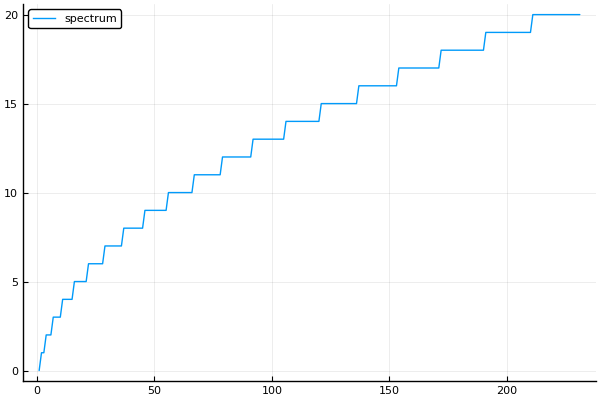
\includegraphics[width=.95\linewidth]{Spc0.png}
      \caption{$\xi = 0$}
      \label{fig:sub1}
    \end{subfigure}%
    \begin{subfigure}{.5\textwidth}
      \centering
      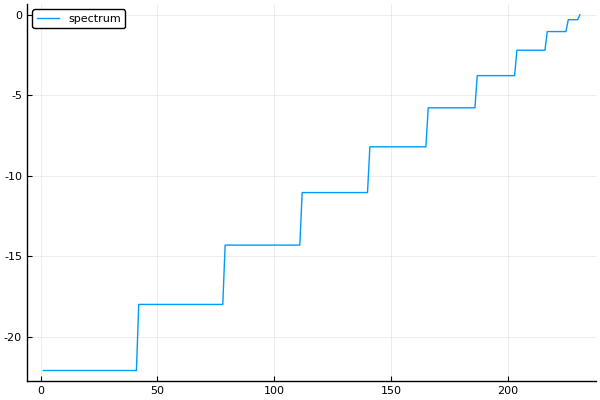
\includegraphics[width=.95\linewidth]{Spc1.png}
      \caption{$\xi = 1$}
      \label{fig:sub2}
    \end{subfigure}
    \caption{Spektra pro $N = 0$ bez vnější poruchy. Na ose x je pořadí hladiny, na ose y je energie.}
    \label{fig:test}
    \end{figure}

Míra degenerace (počet degenerovaných hladin - rozdíl počtu hladin v původním spektru a počtu hladin ve spektru, kde se každé dvě hladiny liší alespoň
o $10^{-13}$) v závislosti na $\xi$ i síle vnější poruchy $\epsilon$ je na obrázku 2.

\begin{figure}[H]
    \centering
    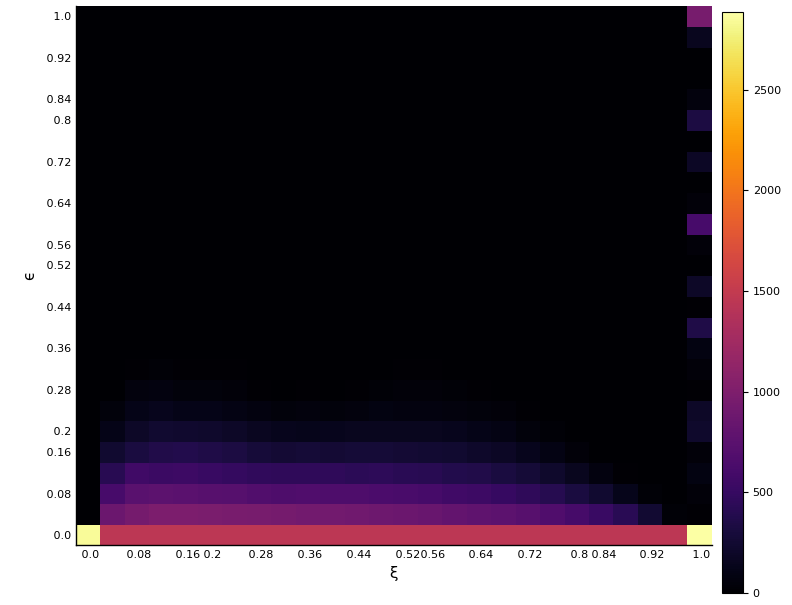
\includegraphics[width=.75\linewidth]{Deg.png}
    \caption{Počet degenerovaných hladin  (počet degenerovaných hladin = rozdíl počtu hladin v původním spektru a počtu hladin ve spektru, kde se každé dvě hladiny liší alespoň
    o $10^{-13}$) v závislosti na $\xi$ i síle vnější poruchy $\epsilon$. $N = 75$}
  \end{figure}

\begin{itemize}
    \item \textbf{Krajní body} - výrazná degenerace v bodech $\epsilon = 0$ a $\xi = 0\,\text{a}\,1$ je kvůli dodatečné symetrii (obrázek 1)
    \item \textbf{Mezioblast} - pro $\epsilon = 0$ máme mezi krajními body $\xi$ degeneraci v párech $l$ a $-l$. V hamiltoniánu je $\hat{l}^2$ a 
    a příspěvek od $\hat{W}$ nezávisí na znaménku $l$.
    Jen $l = 0$ netvoří páry, takže počet degenerovaných hladin je 
    $$ \frac{1}{2}\bigg( \frac{(N+1)(N+2)}{2} - (\floor*{\frac{N}{2}} + 1) \bigg), $$
kde $\floor*{x}$ je spodní celá část. Pro  $\epsilon = 0$ jde tak o skutečnou degeneraci. Po diagonalizaci však rodíly degenerovaných hladin 
leží v intervalu $[0,10^{-13}]$.

S rostoucím $\epsilon$ dochází k rozbití degenerace. Velikost oblasti s degenerací ale závisí na $N$, viz obrázek 3. Degenerované zůstávají
hladiny s velkými $l$. S rostoucím $N$ máme i hladiny s vyšším $l$. Tato degenerace vypadá jen jako numerická chyba. 

    \item \textbf{Krajní oblast} - se změnou poruchy se objevují spárované hladiny ve spektru. Asi také jen numerické
\end{itemize}



  \begin{figure}[H]
    \centering
    \begin{subfigure}{.5\textwidth}
      \centering
      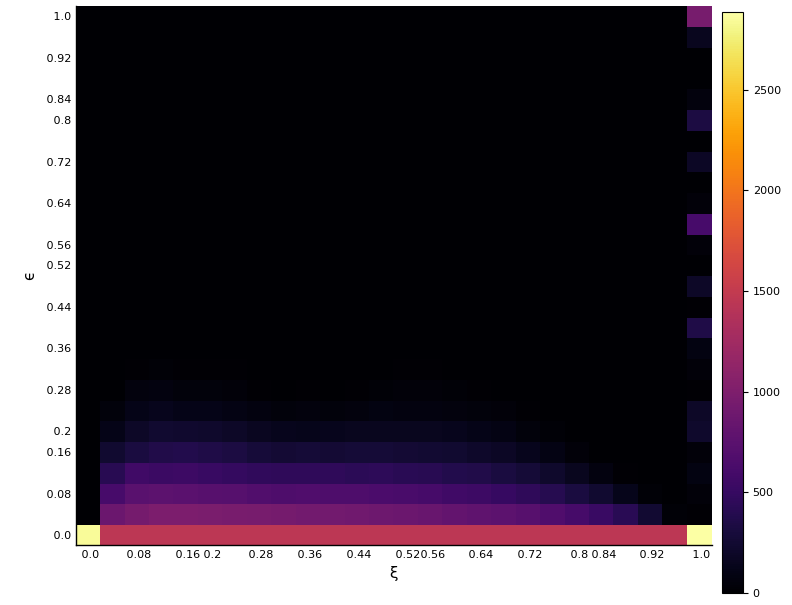
\includegraphics[width=.95\linewidth]{Deg.png}
      \caption{$N = 75$}
      \label{fig:sub1}
    \end{subfigure}%
    \begin{subfigure}{.5\textwidth}
      \centering
      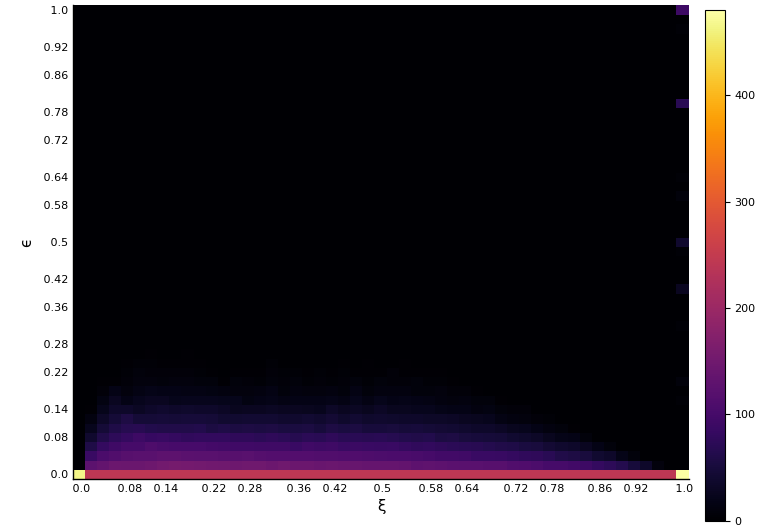
\includegraphics[width=1.05\linewidth]{Deg2.png}
      \caption{$N = 30$}
      \label{fig:sub2}
    \end{subfigure}
    \caption{Porovnání oblastí s degenerací (nalevo sahá až do $\epsilon \approx 0.28 \pm 0.04$ a napravo do $\epsilon \approx 0.20 \pm 0.01$)}
    \label{fig:test}
    \end{figure}


Pár spekter jen v příloze (interaktivní z Plotly).




\end{document}
